\documentclass[a4paper,11pt,dvipsnames]{book}
\renewcommand{\familydefault}{\sfdefault}

\usepackage{standalone}
\usepackage[english]{babel}
\usepackage[top=3cm]{geometry}
\usepackage{float}
\usepackage{tabularx}
\usepackage{multirow}
\usepackage{booktabs}
\usepackage{pgfplots}
\usepackage{amsmath}
\usepackage{amssymb}
\usepackage{amsfonts}
\usepackage{siunitx}
\usepackage{tikz}
\usepackage{graphics} % for pdf, bitmapped graphics files
\usepackage{graphicx}
\usepackage{exsheets}
\usepackage{algorithm}
\usepackage{algorithmicx}
\usepackage[noend]{algpseudocode}
\usepackage{hyperref}
\usepackage{enumitem}
\usepackage{filecontents}
\usepackage{multirow}
%\usepackage{showframe}% to show frames
%\ifCLASSOPTIONcompsoc
\usepackage[caption=false, font=normalsize, labelfont=sf, textfont=sf]{subfig}
%\else
%\usepackage[caption=false, font=footnotesize]{subfig}
%\fi    

\usetikzlibrary{patterns,arrows,arrows.meta,calc,intersections,shapes,positioning,decorations.pathreplacing,decorations.markings,decorations.pathmorphing}
\usepackage{multicol}

\sisetup{output-decimal-marker={,},exponent-product=\cdot}

\DeclareSIUnit\atm{atm}
\DeclareSIUnit\dioptre{D}



\def\BState{\State\hskip-\ALG@thistlm}


\definecolor{TitleColor}{rgb}{0.65,0.04,0.07}
\definecolor{NumberColor}{rgb}{0.02,0.04,0.48}

\DeclareInstance{exsheets-heading}{fancy}{default}{
toc-reversed = true ,
indent-first = true ,
vscale = 2 ,
pre-code = \IfInsideQuestionT{\rule{\linewidth}{1pt}} ,
post-code =\IfInsideQuestionT{\rule{\linewidth}{1pt}} ,
subtitle-format = \large\scshape\color{rgb:red,0.65;green,0.04;blue,0.07} ,
number-format = \large\bfseries\color{rgb:red,0.02;green,0.04;blue,0.48} ,
points-format = \itshape ,
join = { number[r,B]title[l,B](.333em,0pt);
title[r,B]subtitle[l,B](1em,0pt)
} ,
attach =
{
main[hc,vc]number[hc,vc](0pt,0pt) ;
main[l,vc]subtitle[hc,vc](\marginparsep,0pt)
}
}



\DeclareInstance{exsheets-heading}{block-subtitle}{default}{
vscale = 2 ,
pre-code = \rule{\linewidth}{1pt} ,
post-code = \rule{\linewidth}{1pt} ,%title-format = \large\scshape\color{TitleColor} ,
number-format = \large\bfseries\color{rgb:red,0.02;green,0.04;blue,0.48} ,
subtitle-format = \large\scshape\color{black} ,
join = {
title[r,B]number[l,B](.333em,0pt) ;
title[r,B]subtitle[l,B](1em,0pt)
} ,
attach = {
main[l,vc]title[l,vc](0pt,0pt) ;
main[r,vc]points[l,vc](\marginparsep,0pt)
},
}

\DeclareQuestionClass{textbook}{textbooks}

\SetupExSheets{
  headings = fancy,
  question/print = true ,
  solution/print = false }
 % counter-format = se.qu ,
%  counter-within = section ,
  %question/pre-hook = \rule{\textwidth}{1pt},


\hypersetup{
	colorlinks = true, 
	breaklinks = true, 
	bookmarks = true,
	bookmarksnumbered = true,
	urlcolor = blue, 
	linkcolor = blue, 
	citecolor=blue,
	linktoc=page, 
	pdftitle={}, 
	pdfauthor={\textcopyright Author}, 
	pdfsubject={}, 
	pdfkeywords={}, 
	pdfcreator={pdfLaTeX}, % PDF Creator
	pdfproducer={IEEE} }





\tikzset{point/.style={circle,fill,black!80,inner sep=0pt,minimum size=#1,opacity=0.9}}
\tikzset{point/.default=3pt}\tikzset{vector/.style={line width=1pt,postaction={decorate,decoration={markings,mark=at position 1 with {\arrow{latex}}}}}}
\tikzset{block/.style={rectangle,fill=black!30,draw,minimum size=#1,opacity=0.9,align=center}}
\tikzset{block/.default=15pt}\tikzset{ball/.style={circle,fill=black!30,draw,minimum size=#1,opacity=0.9}}
\tikzset{ball/.default=5pt}\tikzset{pulley/.style={draw=black,line width=0.2pt,circle,minimum size=#1,inner sep=0pt,fill=black!10}}
\tikzset{pulley/.default=20pt}\tikzset{rod/.style={line width=2pt}}
\tikzset{rope/.style={line width=1pt}}
\tikzset{spring/.style={decorate,decoration={coil,amplitude=5pt,segment length=#1,aspect=0.3}}}
\tikzset{spring/.default=5pt}\tikzset{wall/.style={black!10,pattern=north east lines,opacity=0.3}}
\tikzset{ray/.style={line width=0.8pt,postaction={decorate,decoration={markings,mark=at position 0.5 with {\arrow{>}}}}}}
\tikzset{arrow/.style={-latex}}
\tikzset{object/.style={line width=1pt,orange,-latex}}
\tikzset{image/.style={line width=1pt,blue,-latex}}
\tikzset{doublearrow/.style={<->,>=latex,thick}}
\tikzset{brace/.style={decorate,decoration={brace,amplitude=#1}}}
\tikzset{brace/.default=5pt}




\graphicspath{{images/}} 




\makeatletter
\@addtoreset{question}{section}
\makeatother


\begin{document}
\author{Dr. Muhammed Rushdi \and Asem Alaa}

\title{Measurements and Instrumentation [SBE206A] (Fall 2018)\\ Tutorial 8}

\maketitle


\chapter*{Descriptive Statistics for Measurements Errors}

\twocolumn

\section*{What is a distribution?}
\begin{enumerate}
\item A probability distribution is a mathematical function that can be thought of as providing the probability of occurrence of different possible outcomes in an experiment\\ \href{https://en.wikipedia.org/wiki/Probability_distribution}{wiki/Probability\_distribution}.
\item A distribution is a function linked to the underlying observations.
\item A distribution provides the probability that an observation has a specific value.
\end{enumerate}

\section*{Visualizing distributions}

\begin{itemize}
\item Discrete distributions are represented by bar charts, where the sum of all bar heights adds up to 1.
\item Continuous distributions are visualized by a curve (probability density function). 
\begin{enumerate}
\item The probability of an exact value (on the x axis) is 0, and there is an unlimited amount of numbers. 
\item Probability is quantified as the area under the curve between two numbers: $$\rm P(a < x < b) $$
which equals the shaded area; calculated by integration.
\item The total area under the curve is 1.
\end{enumerate}
\item Both distributions can be accurately represented by a histogram, or frequency graph.
\item The amount of intervals visualized in a histogram can be computed using \emph{Sturges'} rule:
\begin{equation}
k = \lceil \log_2 n \rceil+ 1
\end{equation}
\end{itemize}



\subsection*{Normal distribution}

\begin{itemize}
\item Defined by the probability density function $$p(x) = \frac{1}{\sigma\sqrt{2\pi}}e^{(-\frac{(x-\mu)^2}{2\sigma^2})}.$$
\item For a normal distribution, the probability of an observation falling between the mean and 1 $\sigma$ away is 34.1\%. Probability of falling between $-2\sigma$ and $+2\sigma$ is 95.4\%.
\end{itemize}

\section*{Z-score}
\begin{itemize}
\item Percentage of observations between standard deviations: -1 to 1: 68.2\%, -2 to 2: 95.4\%, -3 to 3: 99.8\%.
\item Z-score is defined as $Z = \frac{x-\mu}{\sigma}$. It is the amount of standard deviations that a point $x$ is away from the mean $\mu$.
\item Applied to all values, this procedure transforms the data to have $\mu=0$ and $\sigma=1$. A distribution with such mean and standard deviation is said to be normalized.
\item Standard normal probability tables can be used to find probabilities.
\end{itemize}


\section*{Random Variables}
The \emph{probability density function} (pdf) of a continuous \emph{Random Variable} is given by 
$$\int_{x_1}^{x_2}f_X(x)dx=P(x_1\leq X\leq x_2), \quad \forall x_1,x_2$$
And satisfies the following properties:
\begin{enumerate}
\item $f(x)\geq 0 \quad \forall x$
\item $\int_{-\infty}^{\infty}f(x)dx=1$
\end{enumerate}

The \emph{Cumulative Distribution Function}(cdf) for a continuous \emph{Random Variable} is 
$$F_X(x)=P(X \leq x) = \int_{-\infty}^{x}f_X(u)du, \quad \forall x$$
And satisifes the following property:
\begin{enumerate}
\item $\frac{\partial F_X(x)}{\partial x}=f_X(x)$ provided that $F'$ exists and $X$ is a continuous \emph{Random Variable}
\end{enumerate}


\section*{Sample Statistics}

\subsection*{Mean, Median, Mode}
\begin{itemize}
\item Sort data ascendingle when calculating these statistics, and keep duplicates if duplicates are present in the data.
\item For a right-skewed distribution, the median is to the right of the mean, and the mode is to the right of the median. To remember the order: the 3 statistics are in alphabetical order for a left-skewed distribution.
\item The median is usually not affected by outliers as much as the mean.
\end{itemize}

Central Tendency: sample average/mean 
$$\bar{x}=\frac{\sum\limits_{i=1}^{n} x_i}{n}$$

Scatter/dispersion: \emph{sample variance} or \emph{sample standard deviation}
$$\hat{\sigma}^2=S^2=\frac{\sum\limits_{i=1}^{n}(x_i-\bar{x})^2}{n-1};$$
$$\quad\hat{\sigma}=S=\sqrt{\frac{\sum\limits_{i=1}^{n}(x_i-\bar{x})^2}{n-1}}$$

\section*{Central limit theorem}

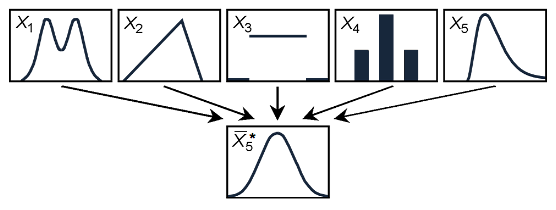
\includegraphics[scale=0.4]{clt}
\begin{itemize}
\item Visualize central limit theory through animation at \href{http://onlinestatbook.com/stat_sim/sampling_dist/index.html}{onlinestatbook.com}
\item If several subsets are taken from an infinite data
population with a Gaussian distribution, then, by the central limit theorem, the means of the subsets will form a Gaussian distribution about
the mean of the infinite data set.
\item The standard deviation of mean values of a
series of finite sets of measurements relative to
the true mean is defined as the standard error
of the mean, $\alpha = \frac{\sigma}{\sqrt{n}}$.
\item The normalized average: 
\begin{equation}
\bar{X_{n}^{*}} = \frac{\bar{X_n} - \mu }{ \sigma / \sqrt{n} }
\end{equation}
$n$ here is the sample size.
\item The interval $x = \bar{X_n} \pm \alpha$ includes the true mean with 68\% certainity. \\
\begin{tabular}{|c|c|}
\hline 
Interval & Confidence \\ 
$\bar{X_n} \pm \alpha$ & 68\% \\ 
$\bar{X_n} \pm 2\alpha$ & 95.4\% \\ 
$\bar{X_n} \pm 3\alpha$ & 99.7\% \\ 
\hline 
\end{tabular} 
\end{itemize}

\section*{Estimation error from a single sample with confidence}

\begin{tabular}{|c|c|}
\hline 
Error & Confidence \\ 
$\pm (\sigma + \alpha )$ & 68\% \\ 
$\pm 1.96(\sigma + \alpha )$ & 95.4\% \\ 
$\pm 3(\sigma + \alpha )$ & 99.7\% \\ 
\hline 
\end{tabular}

\onecolumn

\chapter*{Problems}


\begin{question}
An integrated circuit chip contains 10000 identical transistors. Measurements are made of the current gain of each transistor. Measurements have a mean of 20.0 and a standard deviation of 1.5. The probability distribution of the measurements is
Gaussian.

\begin{enumerate}
\item Write down an expression for the number of transistors that have a current gain between 19.5 and 20.5 and show that this number is approximately 2600 transistor.
\item Calculate the number of transistors that have a current gain of 17 or more (this is the minimum current gain necessary for a transistor to be able to drive the succeeding stage of the circuit in which the chip is used).
\end{enumerate}
\examspace*{10em}

\end{question}
\begin{solution}


\end{solution}


\begin{question}
You collected 29 readings for the pressure drop ($\rm \Delta P$) occurring across a valve in a medical gas network, and computed a sample mean of $\rm \Delta P$ = 2 kPa, along with a
sample standard deviation of $\rm S_{\Delta P}$ = 0.09 kPa. What is the 90\% confidence interval (CI) you would place on the true variance of the pressure drop? (Remember the units)

\examspace*{10em}

\end{question}
\begin{solution}


\end{solution}


\begin{question}
Consider the situation in which a large number of voltage measurements are made. From this data, the mean value of the voltage is 8.5 V and that its variance is 2.25 $\rm V^2$ . The probability distribution of the
measurements is Gaussian.

\begin{enumerate}
\item Determine the probability that a single voltage measurement will fall inside the interval between 10 V and 11.5 V.
\item Determine the probability that no voltage measurement exceeds 15 V.
\end{enumerate}

\examspace*{10em}

\end{question}
\begin{solution}


\end{solution}


\begin{question}
A pressure microsensor is tested by applying a pressure to it of 200 bar, measured by an accurate, calibrated reference pressure-measuring instrument. A set of 12 measurements are made as a reference set of measurements in order to assess the standard deviation and standard error of the mean for measurements made by the device. The measurements obtained for this reference set are: \\
$\left[199.7, 202.0, 200.9, 195.7, 200.2, 199.9, 204.4, 198.0, 203.1, 199.1,  200.5, 196.9\right]$ \\

When the microsensor is subsequently used in a workplace to measure the pressure in an enclosed vessel, a reading of 184 bar is obtained. What is the likely error in this measurement, expressed to
95.0\% confidence limits?

\examspace*{10em}

\end{question}
\begin{solution}


\end{solution}

\begin{question}
You collected 22 readings for air viscosity ($\mu$) in a medical gas network, and computed a sample mean
of $\rm \bar{\eta} = 18.27 ( \rm \mu Pa s)$, along with a sample standard deviation of $\pm 2\%$ of the sample mean. What is the 95\% confidence interval (CI) you would place on the true air viscosity? (Remember the units)

\examspace*{10em}

\end{question}
\begin{solution}

\end{solution}

\begin{question}
A sample of 50000 inductors produced in a factory is taken, and the inductance of each inductor is measured. We want to apply the ${\chi}^2$ test to examine whether the data set formed by the set of 50000
inductors measurements conforms to a Gaussian distribution.
\begin{enumerate}
\item Using the Sturgis rule, show that the number of bins should be set to 17.
\item Assuming that the number of samples in each bin exceeds the minimum threshold, the ${\chi}^2$  statistic was computed to be 7.55. Test whether the measurements follow a Gaussian distribution with significance levels $\alpha$ of 90\% and 95\%, respectively.
\end{enumerate}
\examspace*{10em}

\end{question}
\begin{solution}

\end{solution}


\begin{question}

A certain measurement gave the value of $C_p$, the specific heat of protein, as 1700 J/kg$^{\circ}$C. The precision of measurement is specified by the standard deviation given by 25 J/kg$^{\circ}$C.
If the measurement is repeated what is the probability that the value is within $1700 \pm 40$ J/kg$^{\circ}$C? \\
You may assume that the error is normally distributed.
\examspace*{10em}

\end{question}
\begin{solution}

\end{solution}

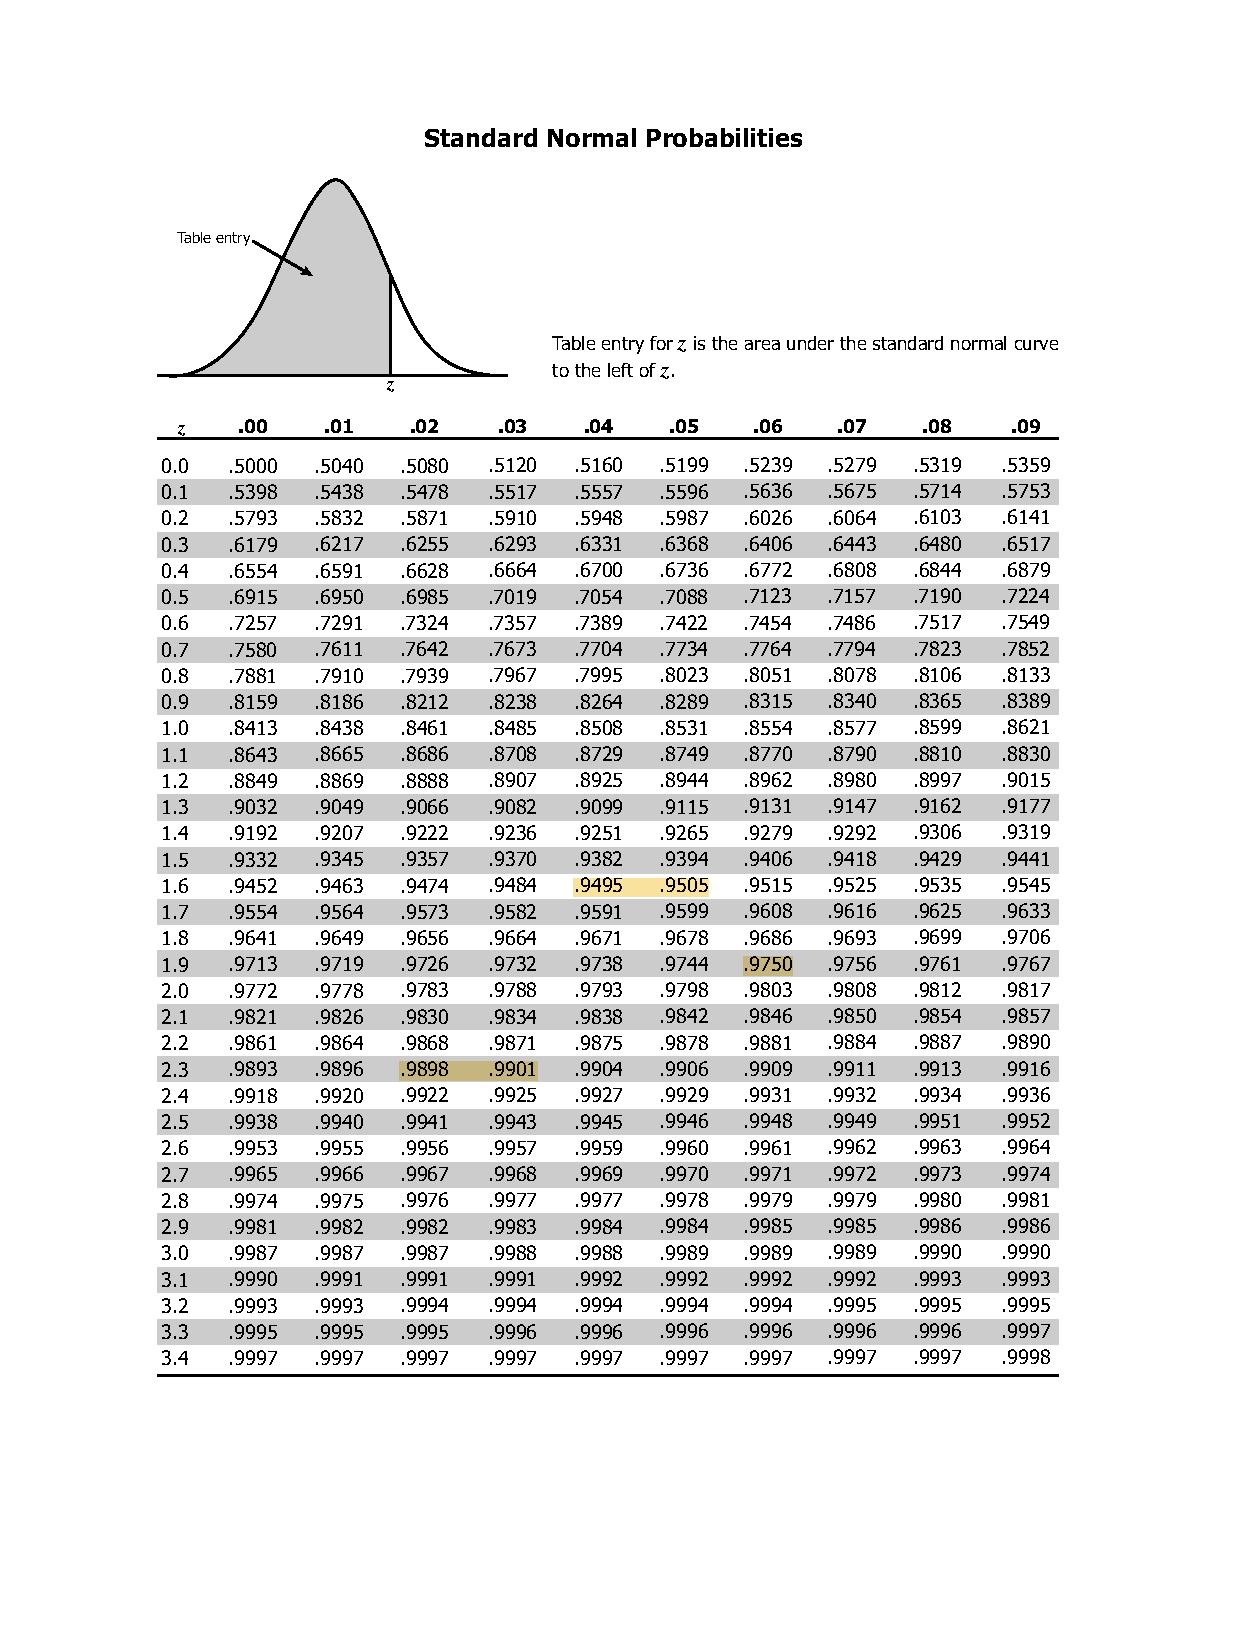
\includepdf[pages=-,pagecommand={},width=1.5\textwidth ]{z-table.pdf}
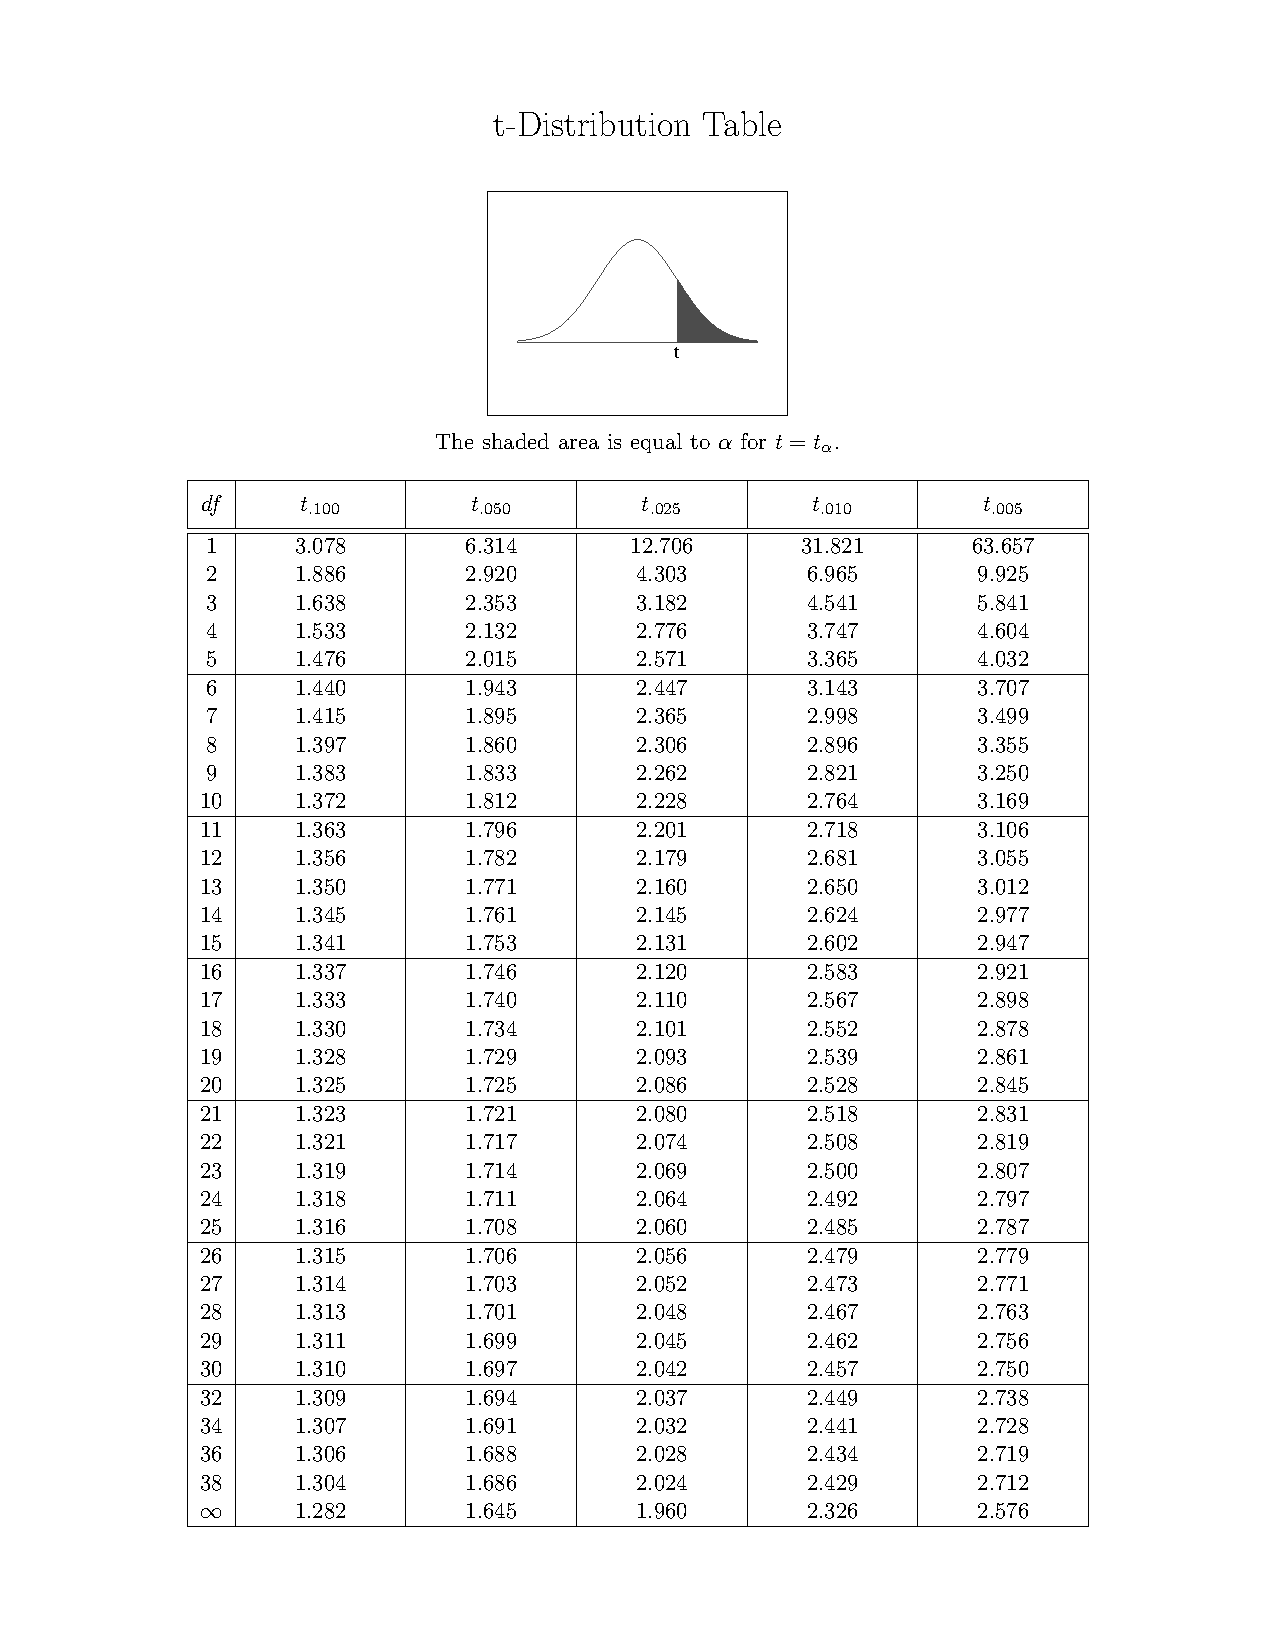
\includepdf[pages=-,pagecommand={},width=1.5\textwidth ]{t-table.pdf}
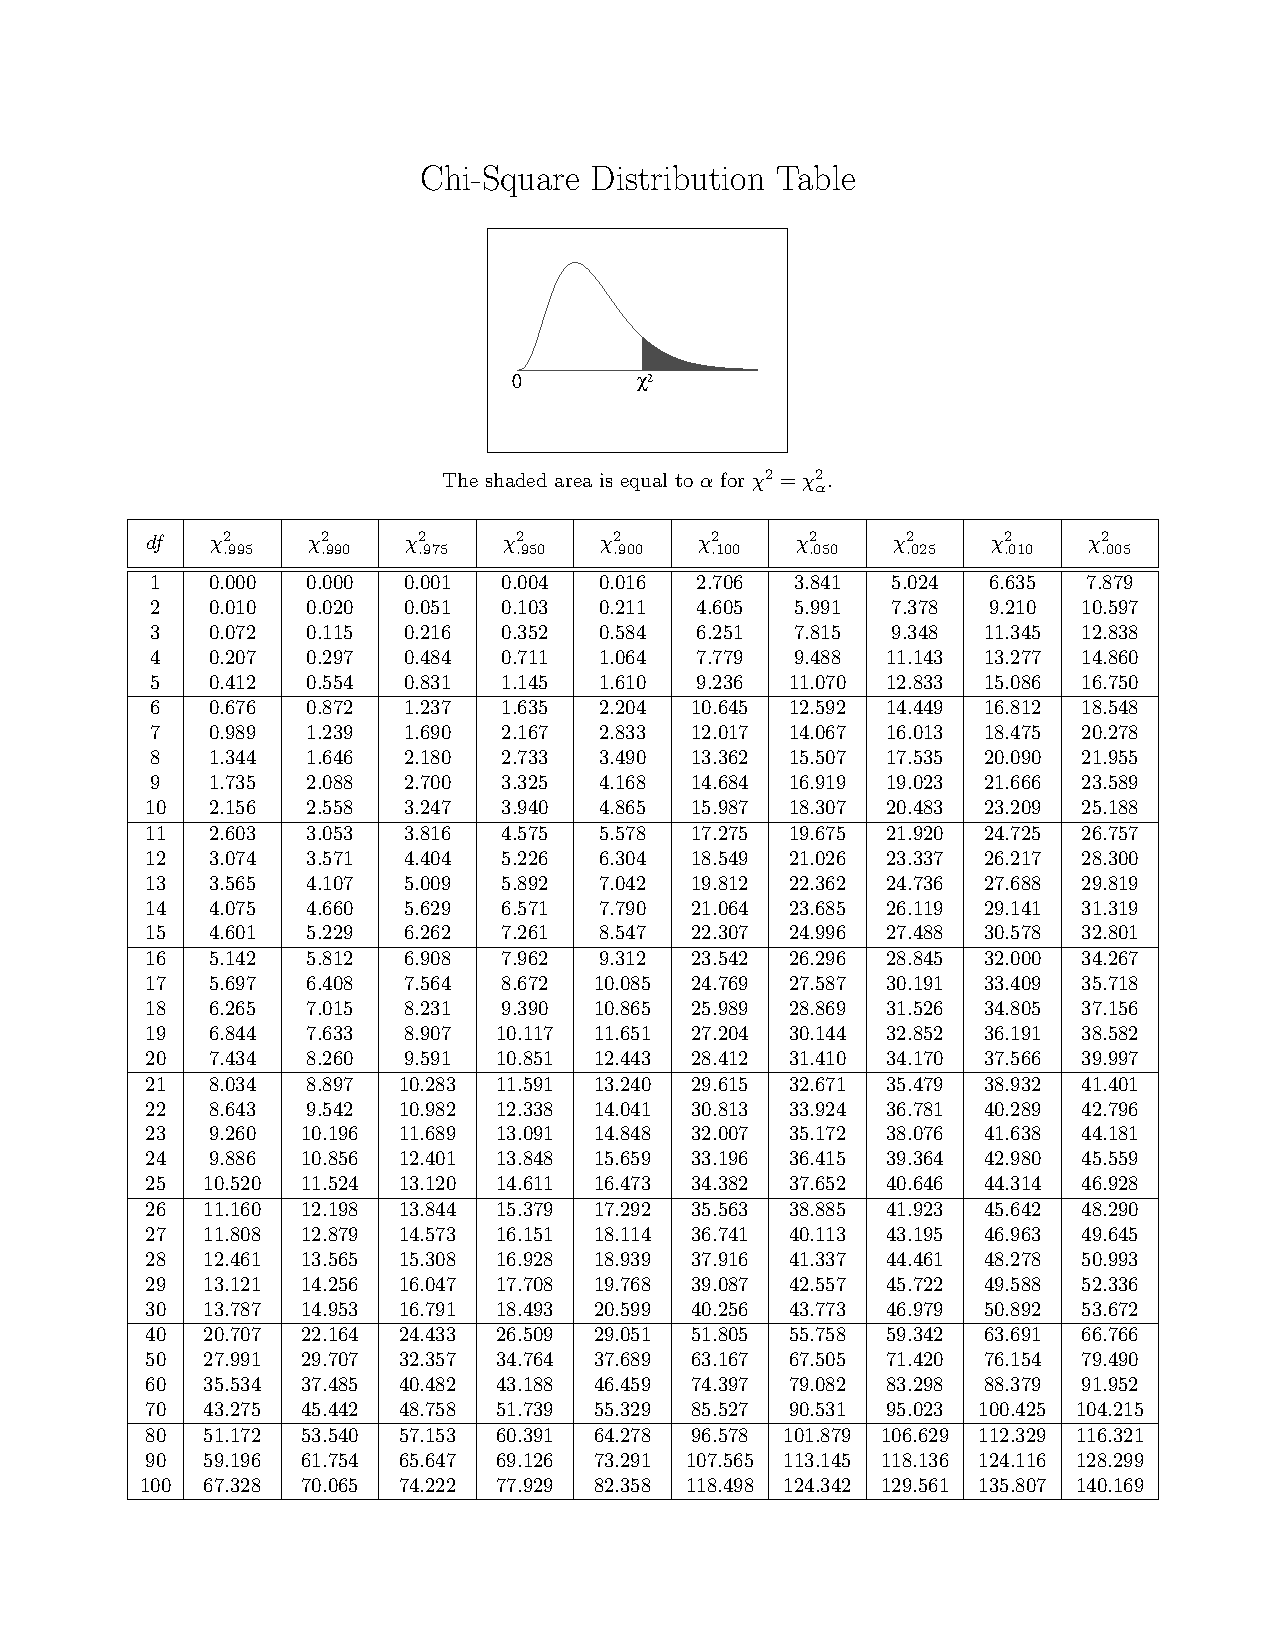
\includepdf[pages=-,pagecommand={},width=1.5\textwidth ]{chi-table.pdf}

\end{document}
